\chapter{Design Objectives}
\label{three}

In this chapter we discuss about our overall goal for using LLVM as a new Parabix back end. First, we show that the IDISA library could be replace by a pure target-independent IR library.

To start, let us look at one IDISA vertical operation: {\tt simd<8>::add}. IDISA library implements this function with the compiler intrinsic that directly translates into the assembly code, so different header files have to be maintained for different instruction sets such as Program~\ref{prog:add_8_sse2} and Program~\ref{prog:add_8_neon}. However, with the LLVM IR, we can implement it as Program~\ref{prog:add_8_llvm}; no low level detail is specified here.

\begin{program}
\begin{verbatim}
  template <> bitblock128_t simd<8>::add(bitblock128_t arg1, bitblock128_t arg2)
  {
    return _mm_add_epi8(arg1, arg2);
  }
\end{verbatim}
\caption{Implementation of {\tt simd<8>::add} for X86 SSE2}
\label{prog:add_8_sse2}
\end{program}

\begin{program}
\begin{verbatim}
  template <> bitblock128_t simd<8>::add(bitblock128_t arg1, bitblock128_t arg2)
  {
    return (bitblock128_t)vaddq_u8((uint8x16_t)(arg1), (uint8x16_t)(arg2));
  }
\end{verbatim}
\caption{Implementation of {\tt simd<8>::add} for ARM NEON}
\label{prog:add_8_neon}
\end{program}

\begin{program}
\begin{verbatim}
  define <16 x i8> @simd_add_8(<16 x i8> %arg1, <16 x i8> %arg2) {
  entry:
    %r = add <16 x i8> %arg1, %arg2
    ret <16 x i8> %r
  }
\end{verbatim}
\caption{Implementation of {\tt simd<8>::add} with LLVM IR}
\label{prog:add_8_llvm}
\end{program}

\begin{program}
\begin{verbatim}
  define <16 x i8> @simd_eq_8(<16 x i8> %arg1, <16 x i8> %arg2) {
  entry:
    %r1 = icmp eq <16 x i8> %arg1, %arg2
    %r2 = sext <16 x i1> %r1 to <16 x i8>
    ret <16 x i8> %r2
  }
\end{verbatim}
\caption[Implementation of {\tt simd<8>::eq} with LLVM IR]{Implementation of {\tt simd<8>::eq} with LLVM IR. {\tt Sext} is the instruction for sign extension.}
\label{prog:icmp}
\end{program}

\begin{program}
\begin{verbatim}
  define <16 x i8> @simd_max_8(<16 x i8> %a, <16 x i8> %b) {
  entry:
    %m = icmp sgt <16 x i8> %a, %b
    %r = select <16 x i1> %m, <16 x i8> %a, <16 x i8> %b
    ret <16 x i8> %r
  }
\end{verbatim}
\caption[Implementation of {\tt simd<8>::max} with LLVM IR]{Implementation of {\tt simd<8>::max} with LLVM IR. {\tt Select} selects elements according to the first operand: $\text{\tt r}_i=
\begin{cases}
    \text{\tt a}_i& \text{if } \text{\tt m}_i = 1\\
    \text{\tt b}_i& \text{otherwise}
\end{cases}$.}
\label{prog:max}
\end{program}

Most of the IDISA vertical operations can be expressed with a few lines of IR code. A bit more examples are listed here:

\begin{itemize}
    \item Vector addition, subtraction, multiplication and shifting. There are IR instructions that correspond one-to-one with them.
    \item Integer comparison such as equality, greater than and unsigned less than. In IR, there is one instruction called `icmp' which does the comparison. The only difference is that for vector type {\tt <N x iX>}, the comparison result of `icmp' is in type {\tt <N x i1>} while IDISA requires it to be in type {\tt <N x iX>} (All ones in an element means true and all zeros means false). We need to perform a sign extension by coping the sign bit of the $i1$ result until it reaches the size of $iX$ (Program~\ref{prog:icmp}).
    \item Operations that have no IR correspondence such as {\tt simd::min} and {\tt simd::max}. They can be emulated with a sequence of IR, e.g.\ {\tt simd<8>::max} in Program~\ref{prog:max}.
\end{itemize}

For horizontal operations, IDISA also needs to maintain target-specific logic. For example, to implement {\tt hsimd<16>::packh}, it uses unsigned saturation $packuswb$ for X86 SSE2 and uses $vuzpq\_u8$ for NEON; for X86 SSE series after SSSE3, it uses the instruction $pshufb$. The author of the IDISA library needs to know these instruction sets very well. On the other hand, LLVM IR introduces a powerful instruction which can express most of the horizontal and expansion operations. It is the \textit{shufflevector}.

\begin{verbatim}
    <result> = shufflevector <n x <ty>> <v1>, <n x <ty>> <v2>, <m x i32> <mask>
    ; yields <m x <ty>>
\end{verbatim}

The first two operands are vectors of the same type and their elements are numbered from left to right across the boundary. In the other word, the element indexes are $0$ \ldots $n-1$ for {\tt v1} and $n$ \ldots $2n-1$ for {\tt v2}. The {\tt mask} is an array of constant integer indexes, which indicates the elements we want to extract to form the {\tt result}. Either {\tt v1} or {\tt v2} can be "undefined" to do shuffle within one vector. Shufflevector is often used together with the \textit{bitcast} operation. It converts between integer, vector and FP-values and changes the data type without moving or modifying the data, thus requiring the source and result type to have the same size in bits. With shufflevector and bitcast, we could write {\tt hsimd<32>::packh} in Program~\ref{program:packh_32}. Figure~\ref{figure:packh_32} explains the indexes used in the shuffle mask.

\begin{figure}[ht!]
\centering
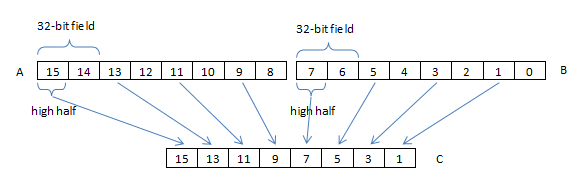
\includegraphics[width=130mm]{draw/packh_16.png}
\caption[Implement {\tt hsimd<32>::packh} with shufflevector]{Shufflevector and {\tt hsimd<32>::packh}. The vectors are bitcasted into $v8i16$ and the indexes for the shuffle mask are drawn in the cell.}
\label{figure:packh_32}
\end{figure}

\begin{program}
\begin{verbatim}
  define <8 x i16> @hsimd_packh_32(<4 x i32> %a, <4 x i32> %b) {
  entry:
    %aa = bitcast <4 x i32> %a to <8 x i16>
    %bb = bitcast <4 x i32> %b to <8 x i16>
    %rr = shufflevector <8 x i16> %bb, <8 x i16> %aa, <8 x i32> <i32 1, i32 3,
          i32 5, i32 7, i32 9, i32 11, i32 13, i32 15>

    ret <8 x i16> %rr
  }
\end{verbatim}
\caption[Shufflevector implementation of packh.]{Shufflevector and {\tt hsimd<32>::packh} in LLVM IR\@. Horizontal operations half the width of fields and that effect is reflected in the return value type.}
\label{program:packh_32}
\end{program}

Program~\ref{program:packh_32} can be easily generalized for packing high on any power-of-two field width. For other horizontal operations:
\begin{itemize}
    \item Packing low: the same bitcast need to be done but shufflevector with a different mask. E.g.\ {\tt hsimd<32>::packl} can be implemented with the mask {\tt 0, 2, 4, 6, 8, 10, 12, 14}.
    \item Packing sign mask: it packs together all the sign bits from each field of the operand. This can be implemented with the less than comparison. E.g.\ {\tt hsimd<32>::signmask(a)} is equivalent to \verb|icmp slt <4 x i32> %a, <4 x i32> <i32 0, i32 0, i32 0, i32 0>| which returns a {\tt <4 x i1>} sign mask vector.
    \item Other operations that require coding a sequence of IR like {\tt hsimd<32>::add\_hl(a, b)}. They are rarely used in the Parabix application.
\end{itemize}

Shufflevector and bitcast could also cover IDISA expansion operations. We list the IR code for {\tt esimd<16>::mergeh} in Program~\ref{prog:mergeh_16} and explain the indexes in Figure~\ref{fig:mergeh_16}. The program is self-explanatory; any programmer who understands shufflevector can understand its behaviour easily.

\begin{figure}[ht!]
\centering
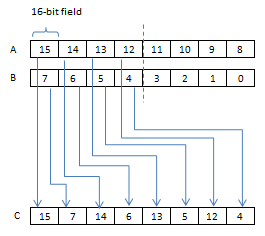
\includegraphics[width=60mm]{draw/mergeh_16.png}
\caption[Implement {\tt esimd<16>::mergeh} with shufflevector]{Shufflevector and {\tt esimd<16>::mergeh}. The indexes for the shuffle mask are drawn in the cell.}
\label{fig:mergeh_16}
\end{figure}

\begin{program}
\begin{verbatim}
  define <4 x i32> @esimd_mergeh_16(<8 x i16> %a, <8 x i16> %b) {
  entry:
    %rr = shufflevector <8 x i16> %b, <8 x i16> %a, <8 x i32> <i32 4, i32 12,
          i32 5, i32 13, i32 6, i32 14, i32 7, i32 15>

    %rr1 = bitcast <8 x i16> %rr to <4 x i32>
    ret <4 x i32> %rr1
  }
\end{verbatim}
\caption[Shufflevector implementation of mergeh.]{Shufflevector and {\tt esimd<16>::mergeh} in LLVM IR\@. Expansion operations double the width of fields.}
\label{prog:mergeh_16}
\end{program}

The rest of the expansion operations can be implemented as the following:
\begin{itemize}
    \item Merge low: similar to merge high but with a different shuffle mask. E.g.\ {\tt esimd<16>::mergel} uses the mask {\tt 0, 8, 1, 9, 2, 10, 3, 11}.
    \item Unary operations like sign extension and zero extension: LLVM has built-in instructions with the same name.
\end{itemize}

For field movement operations:
\begin{itemize}
    \item Field extract or insert: LLVM IR offers two vector instructions {\tt insertelement} and {\tt extractelement} for them.
    \item Constant fill: it fills each field with an integer constant. In IR this can be coded with vector constants such as {\tt <4 x i32> <i32 1, i32 10, i32 30, i32 99>}.
    \item Unary and binary movement: those operations move fields within one register or among two registers and they can be implemented with shufflevector.
\end{itemize}

The full register operations could be coded in large-size integers like $i128$ and $i256$. You can add / multiply / shift it as a normal integer. In fact, all the integer instructions LLVM support can be applied to them thus enabling more complexed operations that IDISA does not support.

To sum up, with support of all the five categories of IDISA operations, we are able to replace the IDISA library with pure IR implementation. However, there is still one question to answer: since LLVM has its own C++ compiler called Clang and Clang could compile the C++ IDISA library into IR, what is the difference between the Clang-generated IR and our hand-written IR library? There are at least three major difference:

\begin{program}
\begin{verbatim}
  define <2 x i64> @hsimd_packh_8(<2 x i64> %a, <2 x i64> %b) #4 {
  entry:
    %0 = bitcast <2 x i64> %a to <8 x i16>
    %1 = tail call <8 x i16> @llvm.x86.sse2.psrli.w(<8 x i16> %0, i32 8) #1
    %2 = bitcast <2 x i64> %b to <8 x i16>
    %3 = tail call <8 x i16> @llvm.x86.sse2.psrli.w(<8 x i16> %2, i32 8) #1
    %4 = tail call <16 x i8> @llvm.x86.sse2.packuswb.128(<8 x i16> %3, <8 x i16> %1) #1
    %5 = bitcast <16 x i8> %4 to <2 x i64>
    ret <2 x i64> %5
  }
\end{verbatim}
\caption{Clang-generated IR for {\tt hsimd<8>::packh} from compiling the IDISA function}
\label{prog:packh_8_sse2_llvm}
\end{program}

\begin{enumerate}
    \item Clang could not remove all the target-dependency from the C++ source. Not every IR instruction are target-independent. For example, IDISA function {\tt hsimd<8>::packh} compiles to Program~\ref{prog:packh_8_sse2_llvm} and all the functions that start with {\tt @llvm.x86.sse2} are only available on X86 SSE2. This is inherent to the use of direct compiler intrinsic in IDISA.
    \newpage

    \item Illegal operations are handled in different level. Compare the following IR implementation for {\tt simd<4>::add}:
      \begin{center}
        \verb|add <32 x i4> %a, %b|
      \end{center}
    With the Clang-generated IR from the IDISA SSE2 file:
      \begin{center}
        \begin{verbatim}
  %and.i.i.i = and <2 x i64> %b, %m0
  %0 = bitcast <2 x i64> %a to <16 x i8>
  %1 = bitcast <2 x i64> %and.i.i.i to <16 x i8>
  %add.i.i10.i = add <16 x i8> %0, %1
  %2 = bitcast <16 x i8> %add.i.i10.i to <2 x i64>
  %3 = bitcast <2 x i64> %b to <16 x i8>
  %add.i.i.i = add <16 x i8> %0, %3
  %4 = bitcast <16 x i8> %add.i.i.i to <2 x i64>
  %and.i.i.i.i = and <2 x i64> %2, %m0
  %and.i.i7.i.i = and <2 x i64> %4, %m1
  %or.i.i.i.i = or <2 x i64> %and.i.i.i.i, %and.i.i7.i.i
  ret <2 x i64> %or.i.i.i.i
        \end{verbatim}
      \end{center}

    Given that addition on $v32i4$ is not supported by this target, the latter implements it with $v16i8$ addition and a few logic operations in the front end level. Target information is required. And even if the latter code is migrated to a target that supports $v32i4$ addition natively, it could not use that ability unless some fancy optimization could recognize the intention behind these 12 lines.

    On the other hand, the former one-line code is not extended until the legalization phase in the back end. The target-specific details are thus left to the back end.

    \item Since the illegal operation is not extended until the back end, more optimizations are available. The high-level intention of the IR instruction is better preserved. Still for {\tt simd<4>::add}, if one of the operand is all zero, the front end could remove the single line of \verb|add <32 x i4>| more easily than removing the 12 lines of code in the Clang-generated IR\@. It is useful for constant combination as well as other peephole optimizations because it simplifies the pattern recognition. We give an example of peephole optimization on the long integer shifting in Chapter~\ref{five}.
\end{enumerate}

This comparison explains our design goal: to replace the IDISA library with a high-level target-independent IR library. It is different from the IDISA approach fundamentally in the way that it tries not to instruct the compiler how to implement this operation, but rather tell what to implement.

The next question would be that could LLVM compile the IR library to efficient machine code? Experiments on X86 tells no. Simple functions that directly respond to native instructions like {\tt simd\_add\_8} in Program~\ref{prog:add_8_llvm} can be compiled correctly, but for some more complexed ones like shufflevector, where no target so far has native support for it, poor machine code might be generated (e.g.\ pack high for 16-bit fields). Furthermore, LLVM does not have good support for vectors of small element, simple code like \verb|add <128 x i1> %a, %b| would generate big amount of memory operations and eight additions on SIMD registers. To achieve a better code generation, we bring many of the strategies from IDISA to LLVM back end. The next two chapters would describe them in detail.

